\section{Packet Streaming} \label{sec:terminologies}

It is important to compare the data reduction techniques fairly in order to systematically study the
resolution-versus-precision tradeoffs among them. One popular approach is to restrict the techniques
to the same data size and compare data quality. It is, however, difficult to enforce that a
multiresolution scheme uses the same amount of data as does a quantization scheme, because the amount
of change in one step of multiresolution simplification may be different from removing one bit in
the quantization of every data sample. To avoid such mismatch of data increment/decrement units, we
model each reduction scheme as a stream of equally sized \emph{packets}. We define a packet as the
smallest unit of data increment/decrement in our framework, where the packet consists of a relatively
small number of bits from a data set. To study the resolution-versus-precision tradeoffs, we
associate a packet with a resolution level and a precision level (i.e., bit plane), so that each
packet can improve either the data's resolution or its precision. In this framework, different
data-reduction schemes become different orderings of packets, and we call the sequence of packets
\emph{stream}. For example, a quantization scheme would stream packets by precision, whereas a
multiresolution scheme would stream packets by resolution. The property of each stream having the
same total number of packets allows us to perform a fair comparison.

In~\Cref{sec:data-streaming-framework}, we discuss the mechanism of converting original data into a
set of packets. \Cref{sec:static-dynamic-streams} describes packet streams that correspond to common
data-reduction schemes. \Cref{sec:data_dep_streams} presents a greedy algorithm that constructs a
reference packet stream for the data and the analysis task at hand. Finally,
\Cref{sec:stream-signature} introduces a novel concept called \emph{stream signature} that can be
used to study and compare the characteristics of different packet streams.

\subsection{Decomposition of Data into Packets} \label{sec:data-streaming-framework}

Each new packet adds to the data's resolution and/or precision. To introduce the concept of
resolution, we use the popular CDF5/3 discrete wavelet transform~\cite{cdf-wavelets}. Although there
exist other transforms that separate signal\pavol{C: signals?} into discrete bands of frequencies/scales/resolutions,
such as the discrete Fourier transform, we choose wavelet transform because wavelet coefficients are
spatially localized. This localization enables spatial adaptivity, allowing finer resolution in
regions that contain sharp features, at the expense of coarser resolution elsewhere. The
hierarchical-Z indexing scheme~\cite{idx2001} also produces a multiresolution representation, but
unlike wavelets, it offers no interpolation mechanism for low-resolution grids. We choose the CDF5/3
wavelet for its balance between simplicity and effectiveness at decorrelating the input signal. It
is also one of the two transforms of choice in the JPEG2000 standard~\cite{jpeg2000}.

The multidimensional wavelet transform can be performed in multiple passes, which eventually results
in the original domain being partitioned into several \emph{subbands}, each of which can be thought
of as a resolution level. One transform pass creates four subbands in 2D and eight in 3D, of which
the first is a smoothed, downsampled version of the original data. The next seven subbands (in 3D)
add fine details in each subset of the dimensions (see~\Cref{fig:pipeline}). A subsequent transform
pass recurses on the first subband created by the previous pass, leaving the other seven subbands
intact. We use $l$ $(0 \leq l < L)$ to index the subbands, with $l = 0$ referring to the coarsest
subband and $L$ denoting the number of subbands. In this paper, we use $L=22$ (in 3D), corresponding
to three transform passes.

For creating packets corresponding to different precision levels, we quantize floating-point wavelet
coefficients to $B$-bit signed integers. For most of the experiments in this paper, $B=16$. This
quantization eliminates the exponent bits, such that every bit (except the sign bit) can be
associated with a bit plane $b$ ($0\leq b < B$), contributing $2^b$ in absolute value to its
coefficient's value. To avoid special treatment of the sign bit, we convert quantized coefficients
from two's complement form to a negabinary form, in which integers are represented in base $-2$,
i.e., $\sum_{i=0}^{B}{c_i(-2)^i}$ with $c_i\in \{0,1\}$. This transformation increases the number of
bit planes by one, to compensate for the absence of the sign bit. In the negabinary form, the higher
indexed bit planes are less significant.

As mentioned earlier, the smallest unit of data in our framework is called a \emph{packet},
following the common practice of reading bits in batches for performance reasons. More precisely, a
packet consists of bits on the same bit plane, from a \emph{block} of negabinary wavelet
coefficients. A block is a $g\times g\times g$ grid of adjacent coefficients on the same subband.
$g$ is always $2$ for the experiments in this paper (we use $g=16$ with larger data sets in the
supplementary marterials). We let $g$ be a constant, so that finer resolution subbands contain more
packets, which means there is a tradeoff between a packet that provides wider (but coarser) coverage
and a packet that provides finer (but more local) details. Every packet comes from a bit plane $b$
and a subband $l$. A packets improves the precision (or resolution) of a region if it comes from a
bit plane (or subband) that has not been streamed before in the region.

A data reduction scheme can be modeled as an ``inverse'' stream of packets, where the original data
contains all packets, and any reduction step removes certain packets based on some criteria (details
in \Cref{sec:static-dynamic-streams}).  These data streams are provided using a client-server model.
At any point, the client is assumed to have received a subset of packets from the server that it
can use to reconstruct the original function (using the inverse wavelet transform). Therefore, to
compare different streams, we can reconstruct the original data using the same number of packets
from each stream, and perform analysis tasks on each of the (approximate) reconstructions. A stream
is better suited for a given analysis task if it produces results that are closer to the ``ground
truth'', i.e., the reference results computed from the original data. \Cref{fig:pipeline} gives a
schematic view of our data streaming model.

\begin{figure}[h]
\centering
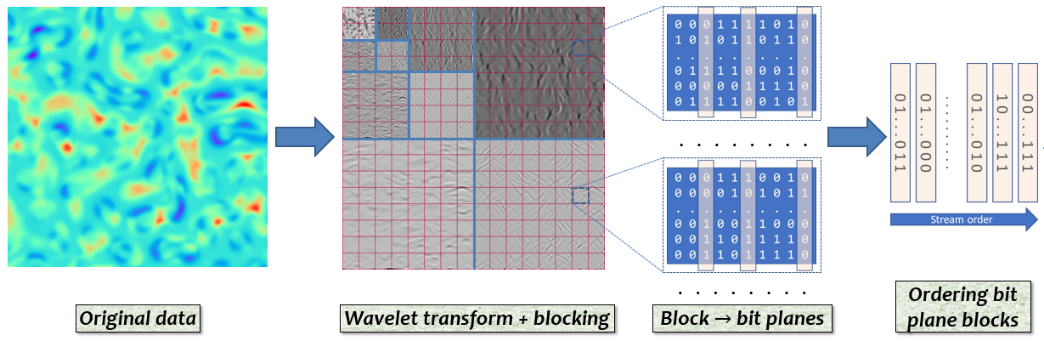
\includegraphics[width=\linewidth]{img/pipeline.png}
\caption{Our data streaming model (in 2D). The input is a regular grid of floating-point samples;
the output is a stream of packets. Different data reduction schemes generate different streams.  The
wavelet subbands are separated by blue lines in the second image, with the coarsest subband at the
top left corner. Although not shown here, quantization and negabinary convesion happen immediately
after wavelet transform. \todo{TODO: revise this figure}}\label{fig:pipeline}
\end{figure}

\subsection{Data-dependent and Data-independent Streams} \label{sec:static-dynamic-streams}

Although both the server and the client in our model can be on the same physical machine, only the
server has full knowledge of the data. Thus, when the client receives a packet, it might not know
where that packet should be deposited. A common solution is to have both the client and the server
agree beforehand on a static ordering of packets, independent of the data. We use the term
\emph{data-independent streams} to refer to streams using this solution. In contrast, for
\emph{data-dependent streams}, an additional mechanism is needed to inform the client about the
position of incoming packets.

A stream is an ordered collection of packets $p_i$ sorted in descending order of some associated
weight $W_i$. Thus, a stream can be characterized using a weighting function. We call the two
sorting criteria, corresponding to two common data reduction schemes in the literature, as \emph{by
level} and \emph{by bit plane}.  The \emph{by level} stream, \slvl, orders the packets strictly from
coarser to finer resolution levels. The weight function in this case is $\wlvl(p)=L-l(p)$, where
$l(p)$ is the subband index of $p$, and $L$ is the total number of subbands. Within the same
subband, without any assumption on the underlying data, packets follow the row-major order of
coefficients and then bit plane order (from 0 to $B$) within each coefficient. The other common
ordering, \emph{by bit plane}, denoted as \sbit, proceeds strictly from higher ordered to lower
ordered bit planes. That is, $\wbit(p)=B-b(p)$, where $b(p)$ is the bit plane index of $p$, and $B$
is the total number of bit planes. Within the same bit plane, packets follow the subband order (from
0 to $L$), and then row-major order in each subband.

The streams \slvl and \sbit are designed to mimic the way data is accessed in traditional methods
that work either in resolution (\slvl) or in precision (\sbit). Additionally, we define a third
stream that combines these two dimensions and refer to it as \emph{by wavelet norm}, \swav.  This
stream orders packets using weights $\wwav(p)=2^{B-1-b(p)}\times \norm{\omega_{l(p)}}^2$. The first
term captures the contribution of a bit on bit plane $b(p)$, and the second term captures the
contribution of a wavelet coefficient on subband $l(p)$, where $\omega_{l(p)}$ refers to a wavelet
basis function on subband $l(p)$. In the wavelet representation, a function $f$ is written as a
linear sum of wavelet basis functions $\omega_i$: $f=\sum{c_i\omega_i}$, where $c_i$ are the
coefficients. Since basis functions in the same subband share the same norm, $\wwav(p)$ is simply
the contribution (in $L_2$ norm) of a bit on bit plane $b_p$ and subband $l_p$, to the whole
function $f$. To our knowledge, a data-reduction scheme based on \emph{by wavelet norm} was hinted
at in~\cite{weiss}.

Another common way to compress wavelet-transformed data is to leave out coefficients of smallest
magnitudes. We model this scheme with a stream called \emph{by magnitude}, \smag. Here, the weight
function is $\wmag(p)=\sum_{c\in \text{block}(p)}\norm{c}^2$ (the sum is over all coefficients in
the block that contains packet $p$). If two packets have the same weight, they are ordered by
subband index, and then by bit plane. Unlike \slvl, \sbit, and \swav, the \smag stream is data
dependent because the coefficient magnitudes are not known before the data has gone through the
wavelet transform.

In theory, data-dependent streams are better than data-independent streams because they can
prioritize important packets based on the actual data. However, data-dependent streams are
ill-suited for practical purposes, because the cost of sending position information likely
outweighs any potential benefit. Nevertheless, we study them for various reasons. First, the
\emph{by magnitude} scheme is well known in the literature. Second, data-dependent streams can serve
as a benchmark to evaluate the performance of their data-independent counterparts. Finally, in
addition to being data dependent, streams can also be task dependent (\Cref{sec:data_dep_streams}),
which may provide insights into how data should be queried to perform certain analysis tasks.

\subsection{Data-dependent, Task-optimized Streams} \label{sec:data_dep_streams}

Each analysis task potentially requires a fundamentally different stream for optimal results.
Studying such an ``optimal'' (and data-dependent) stream is important because it not only serves
as a benchmark, but also can provide insights into other, more practical streams for the same task.

Given the original data set $f$ and its reconstructed approximation $\tilde{f}$ using a subset of
packets, let $q$ represent some quantity of interest\footnote{In this paper, we use the terms
``quantity of interest'' and ``task'' interchangeably, with the understanding that, e.g., if the
task is extracting isosurface, then the quantity of interest is the isosurface.}, e.g., histogram,
isosurface, etc., computed on $f$ or $f'$. For a given task $q$, a well-defined error metric
$\err(q(\tilde{f}),q(f))$ is needed. Given a data set $f$, a task $q$, and an error metric $\err$,
our goal is to generate an \emph{optimal} (and data-dependent) stream, $\sopt$, for $q$ with respect
to $\err$.

We can define $\sopt$ as a stream such that the area under the curve of \err is minimized for all
packets to be streamed. However, this definition is limited in practice because a stream should be
able to terminate at any point and still produce as small an error as possible. Moreover, the
solution to the problem has exponential time complexity.

Instead, we employ a greedy approach to define the optimal stream.  A straightforward greedy
algorithm, however, suffers from the usual limitation of potentially leading to a local optimum. For
example, starting with an all-zero reconstruction $\tilde{f}=0$, and an empty stream, we can
repeatedly append new packets to the stream, which when included in the current $\tilde{f}$, would
minimize $\err$ at every step. Each step might pick a packet that introduces low error, yet
contributes very little to improve the quality of $\tilde{f}$, possibly leading to a nonoptimal
stream at a later point. In order to avoid local minimums, we consider a modification to this greedy
algorithm to build the stream backwards. We start with a ``lossless'' $\tilde{f}$ (i.e.,
$\tilde{f}=f$), and at each step we remove the packet that has the least impact on the error $\err$
from $\tilde{f}$. This modification solves the previous problem where less important packets were
added to $\sopt$ too early. Moreover, it ensures that the packets chosen for removal early on are
indeed less important and will be put at the end of $\sopt$.

Unfortunately, such a greedy algorithm is still expensive in practice, as its complexity is
$\mathcal{O}(n^3)$, with $n$ being the total number of packets in the data. The cubic time
complexity comes from the nested loop ($O(n^2)$) of the algorithm itself, as well as the wavelet
transform ($O(n)$) inside the innermost loop. Considering a $[256 \times 256 \times 256]$ domain, a
packet size that spans $16^3$ coefficients, and $16$ bits of quantization, $n = 65536$, leading to
prohibitively large numbers. Therefore, we adopt a simplified version of this algorithm, where only
one pass through the set of $n$ packets is needed. The modified algorithm works as follows. In each
iteration $i$, we disable (set to zero) a new packet $p_i$ in $\tilde{f}$, and then compute and record
the incurred error $\err_i$. The packet is enabled again in $\tilde{f}$ at the end of iteration $i$.
After $n$ iterations, each packet has an associated weight $\err_i$.  The stream $\sopt$, then, is
simply the sorted list of packets in decreasing order of the weights. This simplified algorithm
brings the running time from days down to hours, while (by observation) retaining the same quality
for $\sopt$. \Cref{alg:greedy} outlines the approach described above.
%\todo{can we use the normal font for the algorithm. why is it so small?}

\begin{algorithm}[h]
  %\small
  %\algsetup{linenosize=\small}
  \caption{Computing a task-optimized stream}
  \begin{algorithmic}[1]
    \Inputs{
			An original function $f$\\
			An unordered set of $n$ packets $P = \{p_i\}$, produced from $f$\\
			A quantity of interest $q$, and an error function $\err$}
		\Initialize{A set of $n$ weights $\Gamma = \{\gamma_i\}$ }
		\For{each packet $p_i$}
			\State $p_i := 0$
      \State $P \rightarrow$ wavelet coefficients $W$ (inverse quantization and inverse negabinary transform)
			\State $W \rightarrow f'$ (inverse wavelet transform)
			\State $\gamma_i := \err(q(f'),q(f))$			
			\State Restore $p_i$
		\EndFor
		\State Sort the $p_i$'s in descending order of $\gamma_i$.
		\Output{The $q$-optimized stream, which is the sorted $P$}
	\end{algorithmic}
	\label{alg:greedy}
\end{algorithm}

\subsection{Stream Signatures} \label{sec:stream-signature}

Unlike data-independent streams, data-dependent streams do not impose a static ordering of packets.
To concisely represent and characterize the dynamic ordering of data-dependent streams, we introduce
the concept of a \emph{stream signature}.  Any data-dependent stream can be represented with respect
to the two-dimensional space of resolution (subbands) and precision (bit planes), i.e., \mbox{$\strm
= \strm_{L,B}=\{(l,b)\ |\ 0\leq l < L,\ 0\leq b < B\}$.} 

Given a stream, we define its signature $\sgn_{L,B}$ as the $L \times B$ matrix, whose $(l,b)$
element is associated with $P_{l,b}$---the set of packets belonging to subband $l$ and bit plane
$b$. In particular, $\sgn(l,b)$ is an integer in the range $[0, B\times L)$, and indicates, on
average, the position at which packet $P_{l,b}$ appears in the given stream. For example, the
signature $\sgn=\bigl[ \begin{smallmatrix}0 & 1 & 4\\ 2 & 3 & 5\end{smallmatrix}\bigr]$ indicates
that the stream begins with packets that lie on the first bit plane of the first subband, as
$\sgn(0,0)=0$. Those are followed by packets on the second bit plane of the first subband
($\sgn(0,1)=1$), and then the first bit plane of the second subband ($\sgn(1,0)=2$). Finally, the
last group of packets comes from the third bit plane of the second subband ($\sgn(1,2)=5$). Thus, a
stream's signature shows how the stream traverses the space $\strm_{L,B}$, and highlights the
different resolution-versus-precision tradeoffs among $\sopt$ optimized for different tasks.

To compute a stream signature, we partition the whole domain (not individual subbands) into several
\emph{regions}, compute one signature per region, and average these local signatures. It is only
when packets are relatively well localized that their relative ordering in the $\strm_{L,B}$ space
becomes meaningful. For example, a packet at one corner of the domain may be streamed before one at
an opposite corner, but this fact contains no useful information. We define a region to be the
spatial volume that is covered by a packet in the coarsest subband. Algorithm~\ref{alg:signature}
lists the steps of our approach.

\begin{algorithm}[h]
  % \small
  \caption{Computing a stream signature}
  \begin{algorithmic}[1]
    \Inputs{
			A stream $P=\{p_i\}$\\}
		\Initialize{Per-region signature matrix $A_r:= 0$\\
		Global signature matrix $A := 0$}
		\For{each packet $p_i$ in $P$}
			\State Let $r$, $b$, $l$ be the region, bit plane, and subband that $p_i$ belongs
			\State $A_r(l,b) := A_r(l,b)+i$
		\EndFor
		\For{each region $r$}
			\State Sort the elements of $A_r$
			\State Assign each element of $A_r$ its index after sorting
			\State $A := A+A_r$
		\EndFor
		\State Sort the elements of $A$
		\State Assign each element of $A$ its index after sorting
		\Output{The signature matrix $A$}
	\end{algorithmic}
	\label{alg:signature}
\end{algorithm}

Finally, a signature can be used to construct a ``semi''-data-independent stream, denoted as
$\ssig$. This construction is done by iterating through each element $\sgn(l,b)$ in ascending order,
and adding end\pavol{C: at the end?} of $\ssig$ all the packets in $P_{l,b}$. $\ssig$ is similar to purely
data-independent streams, in that the ordering of packets in the $\strm_{l,b}$ space is
deterministic (governed by the signature). However, this deterministic ordering must be established
between the client and the server through the transmission of the signature. This is not a hurdle in
practice, because the size of the signature is negligible compared to the size of the data itself.
In 3D, assuming 22 subbands and 32-bit quantized coefficients, a signature contains $1408 (=22\times
32\times 2)$ bytes. Stream $\ssig$ is data dependent but otherwise has no element of
spatial-adaptivity; hence it can serve as a bridge when comparing the resolution-versus-precision
tradeoffs between data-independent and data-dependent streams.

\begin{table}[t]
	\caption{Streams defined in this paper}
  \centering
  \begin{tabular}{p{0.15\textwidth}p{0.06\textwidth}p{0.2\textwidth}}
  \hline
  Name & Symbol & Data dependent\\
  \hline
  \emph{by level} & \slvl & No\\
  \emph{by bit plane} & \sbit & No\\
  \emph{by wavelet norm} & \swav & No\\
  \emph{by magnitude} & \smag & Yes\\
	\emph{rmse-optimized} & \sopt & Yes\\
	\emph{rmse signature} & \ssig & Semi\\
	\emph{gradient-optimized} & \sgop & Yes\\
	\emph{gradient signature} & \sgsg & Semi\\
	\emph{Laplacian-optimized} & \slop & Yes\\
	\emph{Laplacian signature} & \slsg & Semi\\
	\emph{histogram-optimized} & \shop & Yes\\
	\emph{histogram signature} & \shsg & Semi\\
	\emph{isosurface-optimized} & \siop & Yes\\
	\emph{isosurface signature} & \sisg & Semi\\
	% flame & fluid dynamics simulation& float32 & x & x & x & x & x & Done\\
	% csafe & fluid dynamics simulation& uint8 & x &  &  & x & x & Done\\
	% enzo-v & fluid dynamics simulation& float32 & x & x &  & x &  & D(work2nd)\\
	% brain & fluid dynamics simulation& uint8 & x &  &  & x & x & Done\\
	% foam & fluid dynamics simulation& uint16 & x & x & x & x & x & Done\\
	% vismale & fluid dynamics simulation& uint8 & x & x & x & x & x & P(rerun)\\
	% karfs	& fluid dynamics simulation& float32 & x & x &  & x & x & Done\\
	% aneurism	& fluid dynamics simulation& uint8 & x & x &  & x & x & Done\\
  % velocityz & hydrodynamics simulation& float64 & x & x &  & x & x & D(main)\\
  \hline
  \end{tabular}\label{tbl:data-sets}
\end{table}